\documentclass[14pt,a4paper]{article}
\usepackage[14pt]{extsizes}
\usepackage[left=1.5cm, right=1.5cm, top=1.5cm, bottom=1.5cm]{geometry}
\usepackage[utf8]{inputenc}
\usepackage[T2A]{fontenc}
\usepackage[english, russian]{babel}
\usepackage{amsmath,amsfonts,amssymb,amsthm,mathtools} 
\usepackage{amsfonts}
\usepackage{amssymb}
\usepackage{titleps}
\usepackage{hyperref}
\usepackage{float}
\usepackage{graphicx}
\usepackage{multirow}
\usepackage{hhline}
\usepackage{wrapfig}
\usepackage{tikz}
\usepackage{pgfplots}
\usepackage{xcolor}
\usepackage{subfig}
\usepackage{upgreek}

\newcommand{\w}[1]{\text{#1}}
\newcommand{\und}[1]{\underline{#1}}
\newcommand{\img}[3]{
	\begin{figure}[H]
	\begin{center}
	\includegraphics[scale=#2]{#1}
	\end{center}
	\begin{center}
 	\textit{#3}
	\end{center}
	\end{figure}
}
\newcommand{\aw}[1]{
	\begin{center}
	\textit{#1}
	\end{center}
	\n
}
\newcommand{\be}[1]{
	\begin{center}
	\boxed{#1}
	\end{center}
}
\newcommand{\beb}[1]{
	\begin{equation}
	\boxed{#1}
	\end{equation}
}
\newcommand{\eb}[1]{
	\begin{equation}
	#1
	\end{equation}
}
\newcommand{\n}{\hfill \break}
\newcommand{\x}{\cdot}
\begin{document}

\section*{Работа 3.2.8}	
	\section*{Релаксационные колебания}
	\subsection*{Андрей Киркича, Б01-202, МФТИ}

\textbf{В работе используются:} стабилитрон СГ-2 (газонаполненный диод) на монтажной панели, магазин ёмкостей, магазин сопротивлений, источник питания, амперметр, вольтметр, осциллограф.

\section*{1. Теоретические сведения}
\begin{figure}[H]
\centering
\subfloat[Вольт-амперная характеристика стабилитрона с последовательно включенным резистором.]{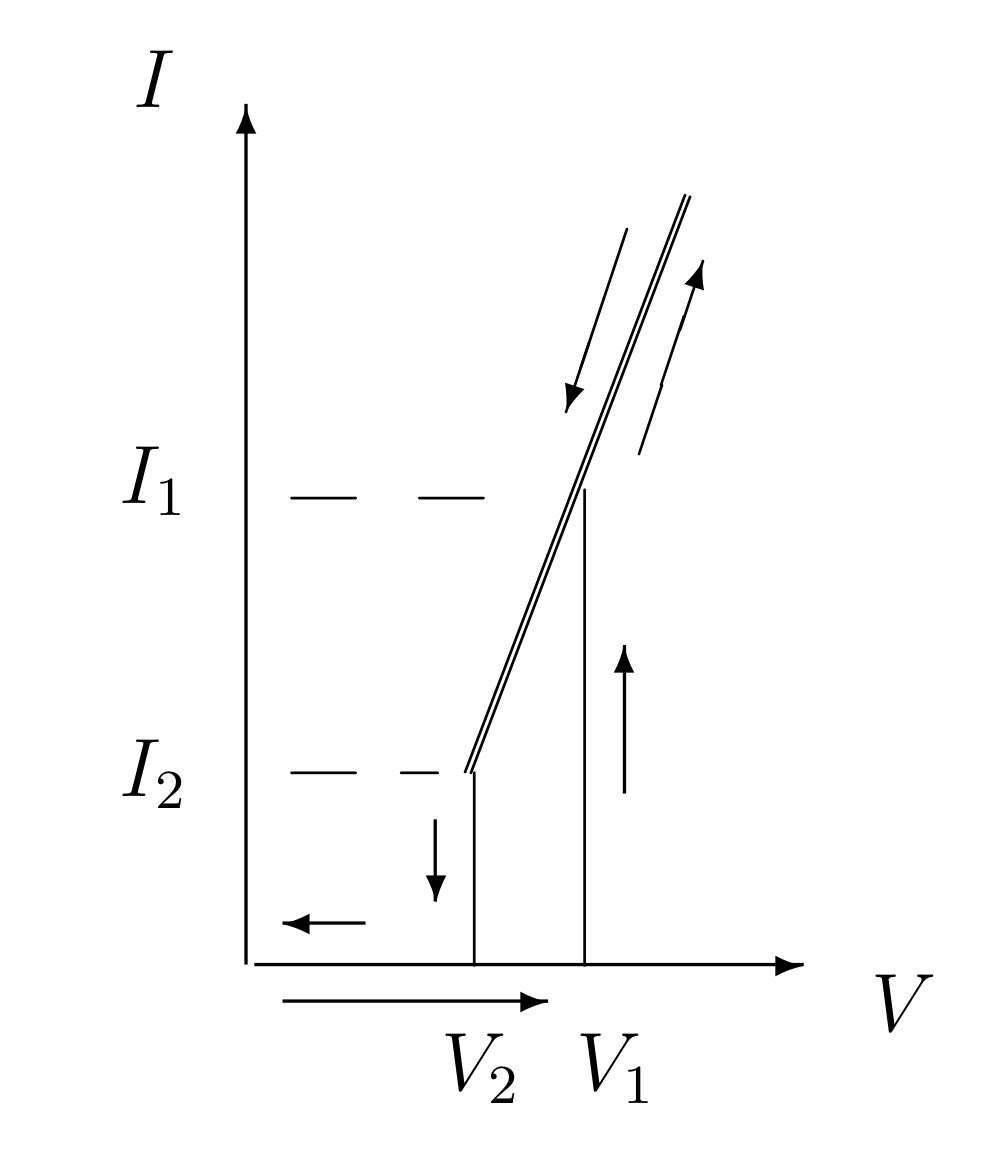
\includegraphics[width=0.3\textwidth]{graph.jpg}}
\qquad \qquad
\subfloat[Cхема релаксационного генератора.]{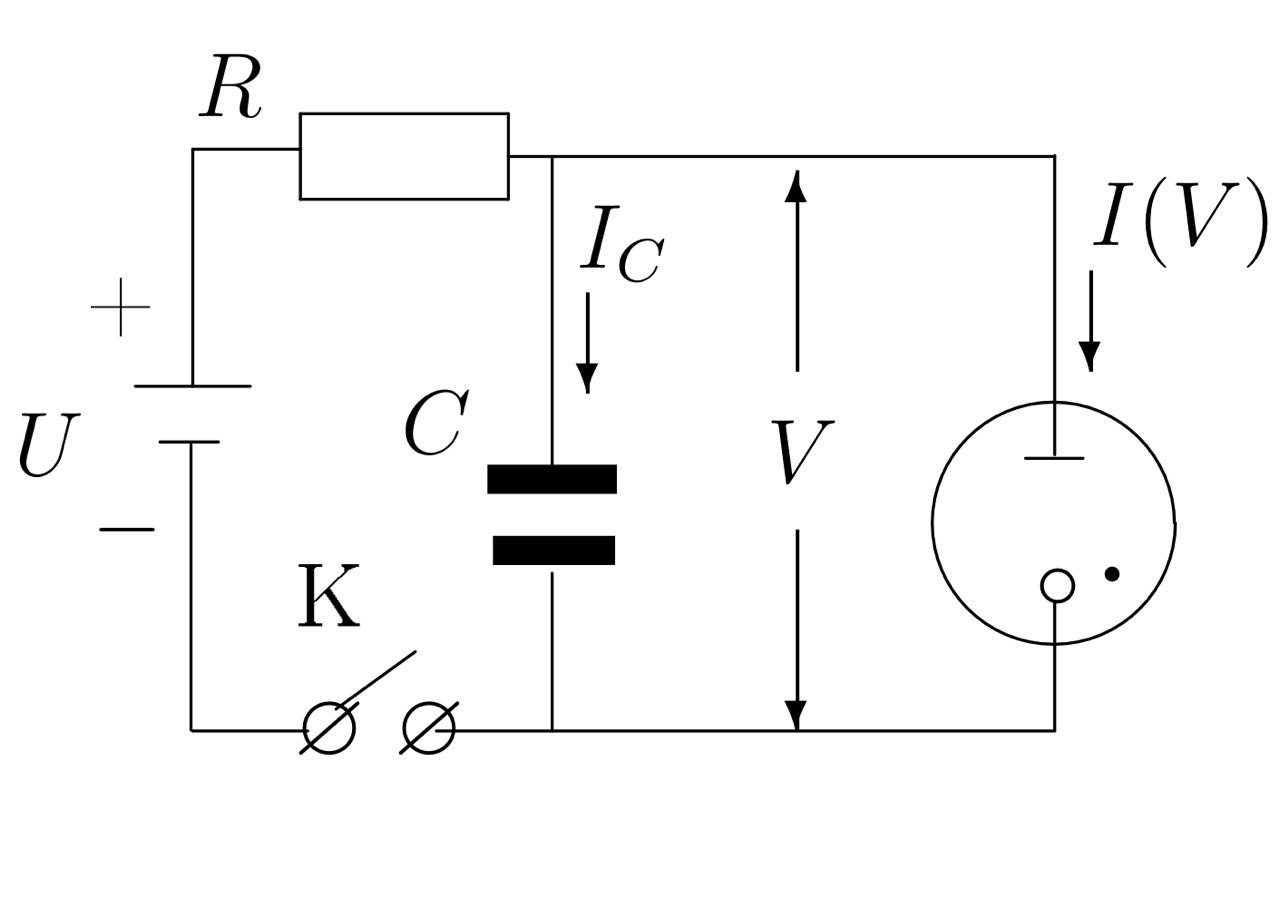
\includegraphics[width=0.4\textwidth]{scheme.jpg}}
\end{figure}

Период колебаний:
\begin{equation}
    T=R C \ln \frac{U-V_{2}}{U-V_{1}},
\end{equation}
Критическое сопротивление:
\begin{equation}
R_{\mathrm{кp}}=\frac{U-V_{2}}{I_{2}}.
\end{equation}

\begin{figure}[H]
\centering
\subfloat[Осциллограмма релаксационных колебаний.]{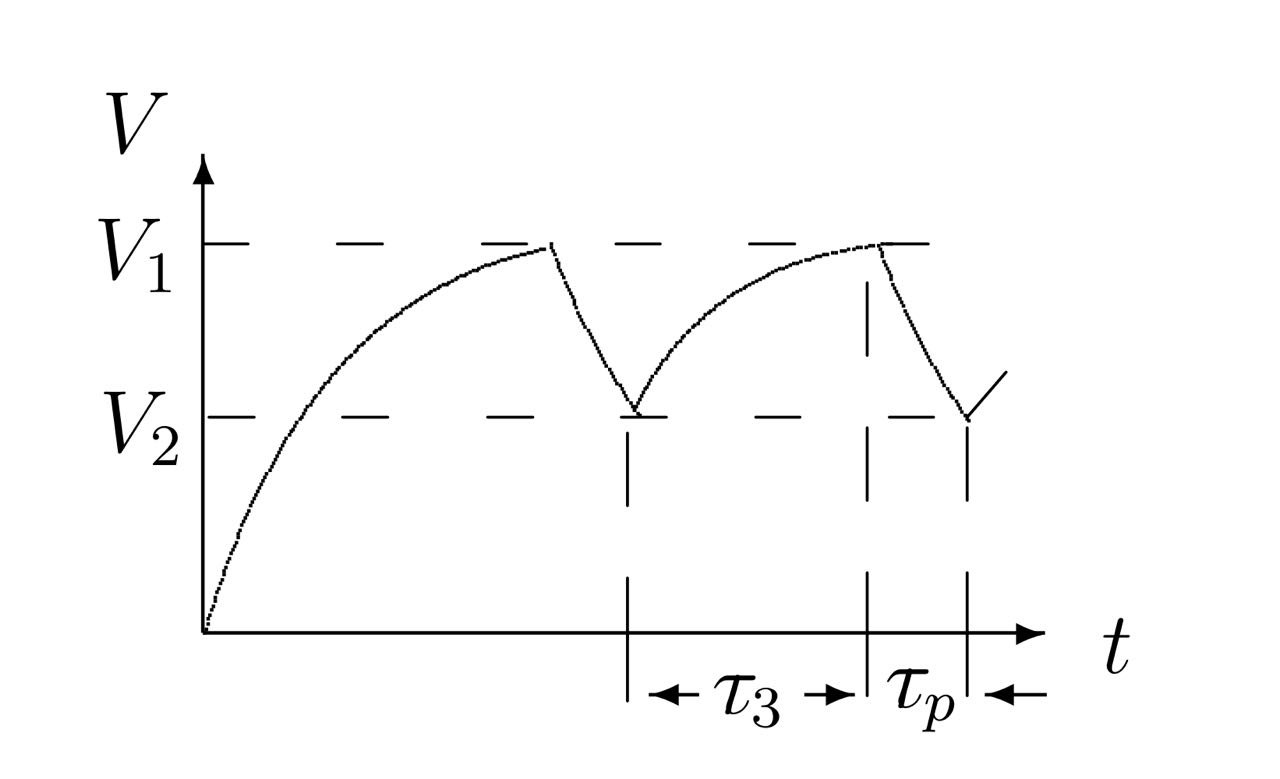
\includegraphics[width=0.4\textwidth]{graph3.jpg}}
\qquad
\subfloat[Схема установки для изучения характеристик стабилитрона.]{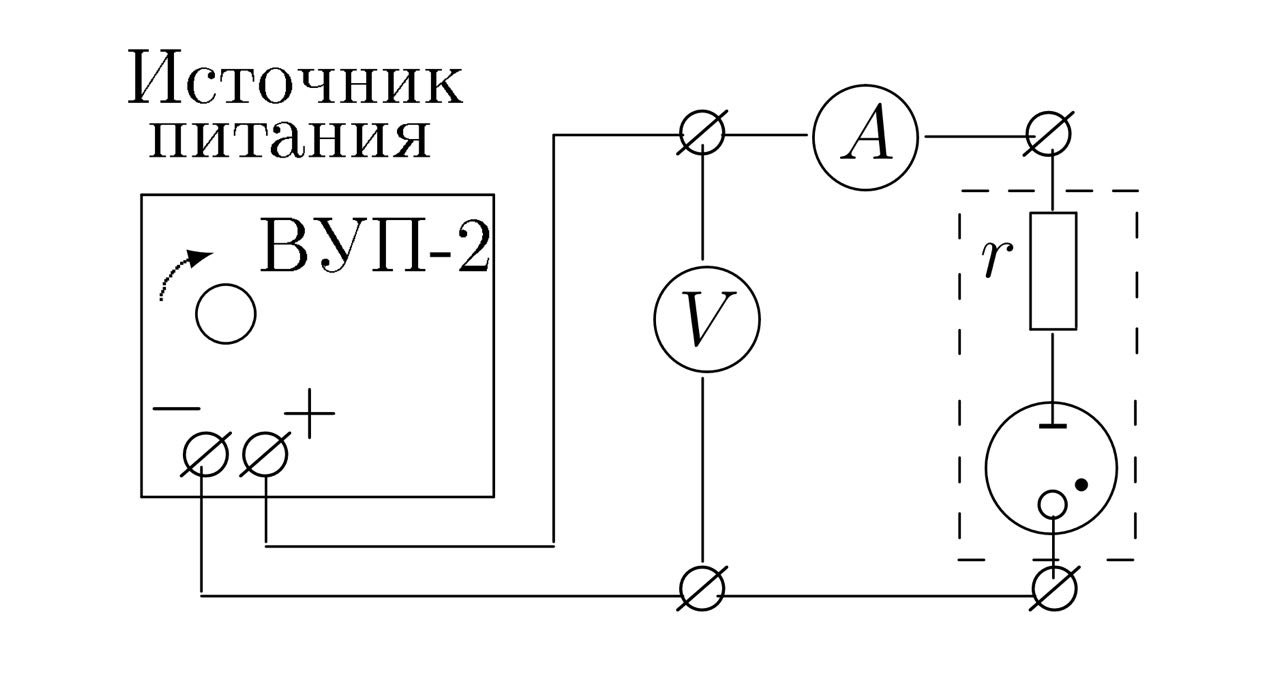
\includegraphics[width=0.4\textwidth]{scheme2.jpg}}
\end{figure}

\section*{2. Результаты измерений}

\subsection*{Характеристика стабилитрона}

Добавочное сопротивление $r = 5,1$ кOм было подпаяно между ножкой лампы и соответствующей клеммой, для того чтобы предохранять стабилитрон от перегорания. Это сопротивление оставалось включённым при всех измерениях. Вольтамперная характеристика стабилитрона с резистором $r$ при возрастании и убывании напряжения представлена в таблице ниже. При этом, для более точного определения потенциалов зажигания и гашения, показания приборов были сняты пятикратно.

\begin{table}[H]
	\centering
    \begin{tabular}{|r|r||r|r|}
	\hline $V$, В & $I$, мА & $V$, В & $I$, мА \\ \hline
	\multicolumn{2}{|c||}{Увеличение напряжения} & \multicolumn{2}{|c|}{Понижение напряжения} \\ \hline
$87,5 \pm 0,5$ & $2,94 \pm 0,05$ & $148,5 \pm 0,5$ & $14,60 \pm 0,05$ \\ \hline
$92,6 \pm 0,5$ & $3,93 \pm 0,05$ & $136,7 \pm 0,5$ & $12,40 \pm 0,05$  \\ \hline
$100,0 \pm 0,5$ & $5,30 \pm 0,05$ & $123,5 \pm 0,5$ & $9,90 \pm 0,05$ \\ \hline
$110,2 \pm 0,5$ & $7,14 \pm 0,05$ & $108,7 \pm 0,5$ & $6,90 \pm 0,05$  \\ \hline
$120,0 \pm 0,5$ & $9,23 \pm 0,05$ & $95,3 \pm 0,5$  & $4,60 \pm 0,05$  \\ \hline
$130,2 \pm 0,5$ & $11,10 \pm 0,05$ & $84,5 \pm 0,5$  & $2,50 \pm 0,05$  \\ \hline
$143,0 \pm 0,5$ & $13,50 \pm 0,05$ & $81,6 \pm 0,5$ & $0,00 \pm 0,05$  \\ \hline
$158,0 \pm 0,5$ & $16,40 \pm 0,05$ & - & - \\ \hline 
    \end{tabular}
    \caption{Вольт-амперная характеристика стабилитрона.}
    \label{voltamp}
\end{table}

По полученным данным был построен график. В качестве напряжений зажигания и гашения были взяты средние значения всех измеренний данных величин.

\begin{figure}[H]
    \centering
    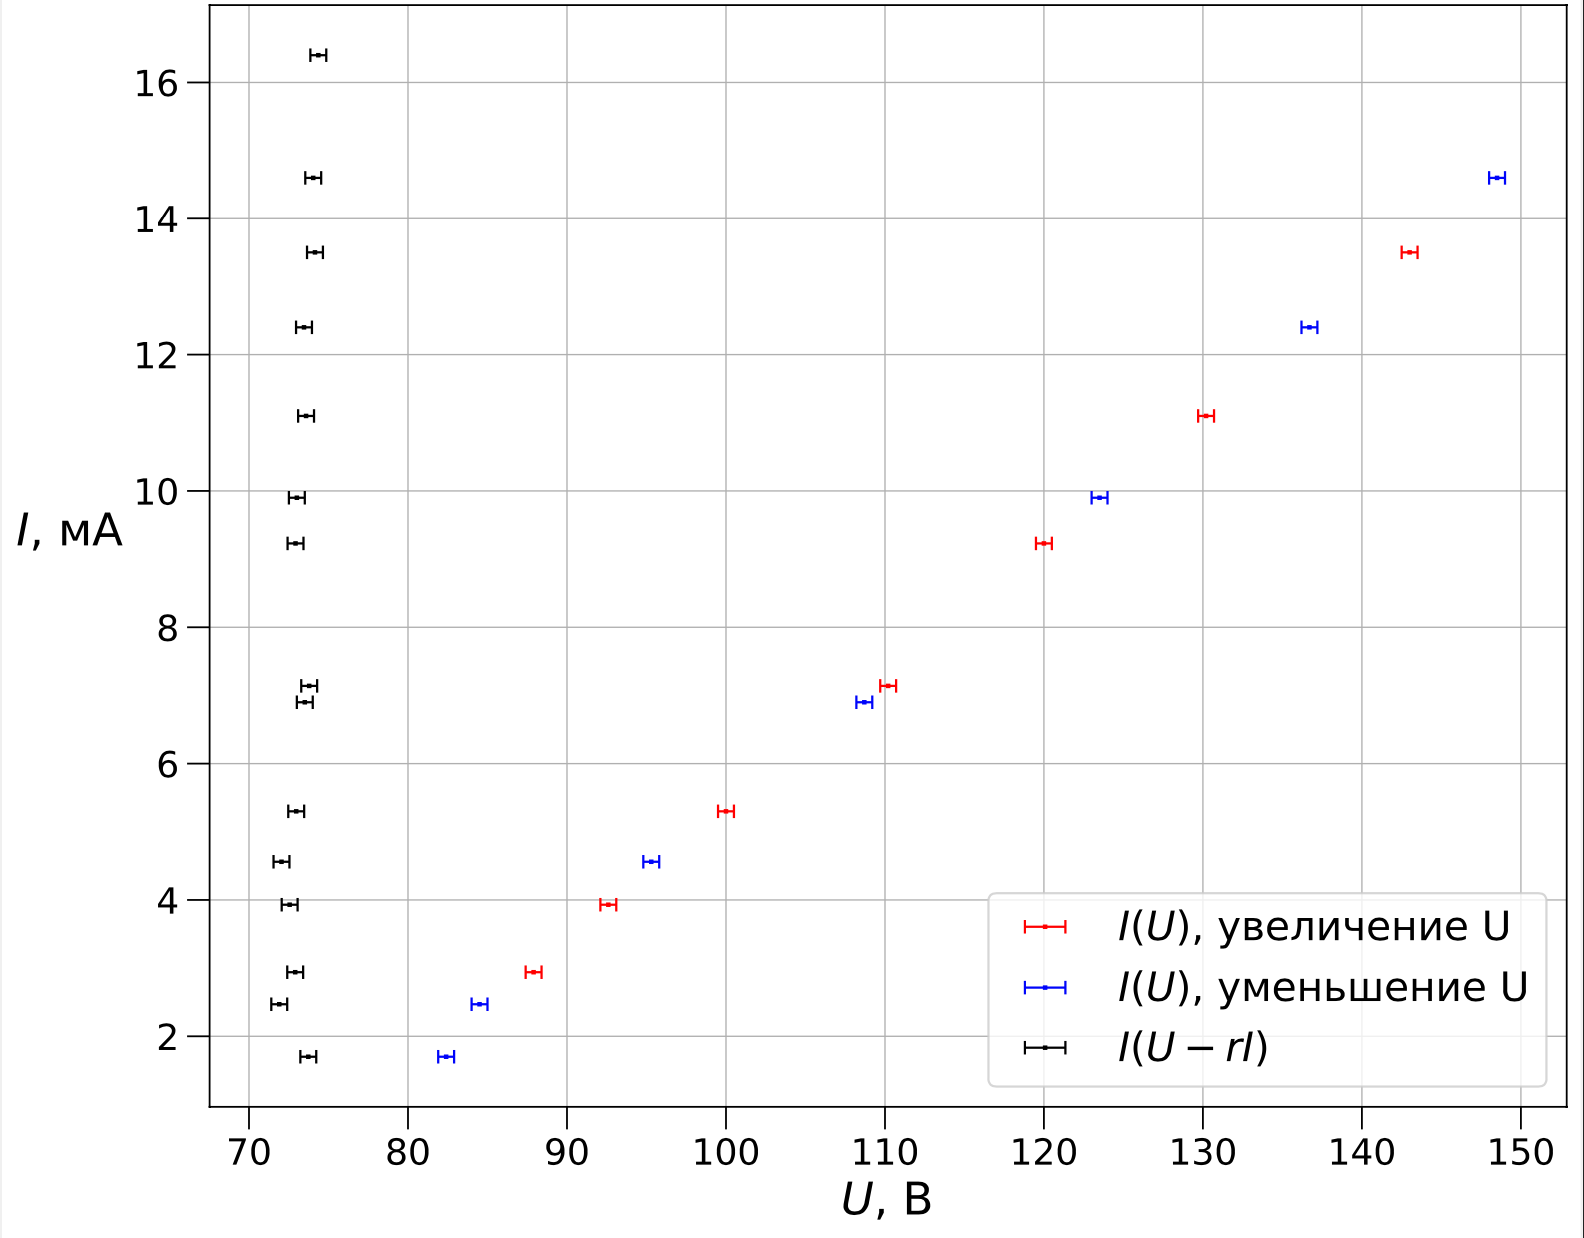
\includegraphics[scale=0.45]{I(U).png}
\end{figure}

\subsection*{Осциллограммы релаксационных колебаний}

Для проведения эксперимента было выставлено напряжение $U = (117,3 \pm 0,5) $В. После подбора частоты развёртки, при которой на экране видна картина пилообразных колебаний, было рассчитано критическое сопротивление по формуле (2): $R_\text{кр} =  (140 \pm 3)$ кОм. Далее была проведена серия измерений для снятия показаний для зависимости $T(C)$. Напряжение при этом было выставлено ($118,0 \pm 0,3$)В, а сопротивление -- $R = 560$ кОм. Результаты измерений приведены в таблице ниже.
\begin{table}[H]
    \centering
    \begin{tabular}{|c|r|r|r|r|r|r|r|}
    \hline $C$, нФ & 50 & 40 & 30 & 20 & 15 & 10 & 5 \\ \hline
    $T$, мс & 26,0 & 21,0 & 15,5 & 10,0 & 7,2 & 4,6 & 2,9 \\ \hline
    \end{tabular}
    \caption{Зависимость периода от электроёмкости.}
    \label{tec}
\end{table}
Ниже приведена зависимость $T(C)$. Помимо этого, по формуле (1) были рассчитаные теоретические значения периода и также отмечены на графике.

\begin{figure}[H]
    \centering
    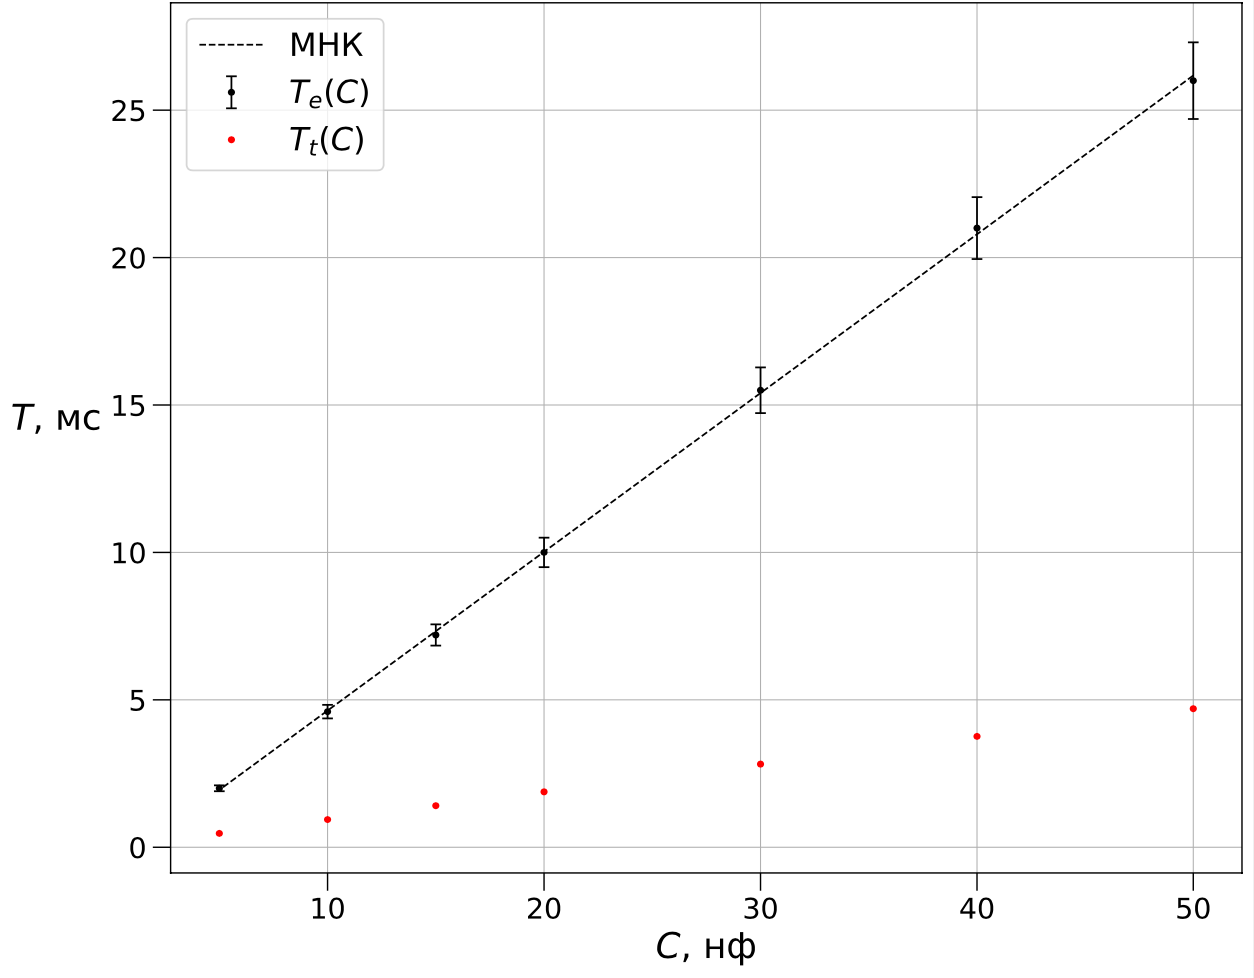
\includegraphics[scale=0.75]{T(C).png}
\end{figure}

Как видно из графика, коэффициенты наклона сильно отличаются, из чего следует, что динамический потенциал отличается от статического. Таким образом, динамический потенциал гашения лампы составил $(42 \pm 6)$ В.

\section*{3. Заключение}

Из вольт-амперной характеристики стабилитрона можем сделать вывод, что стабилитрон работает, и может стабилизировать напряжение. В пределах применения теоретической модели наблюдается прямопропорциональная зависимость периода от ёмкости. 

\subsection*{Литература}

1. \textit{Никулин М.Г., Попов П.В., Нозик А.А., и др.} Лабораторный практикум по общей физике: учеб. пособие. В трёх томах  Т. II. Электричество и магнетизм. - 2-е издание М.: МФТИ, 2019. \n
2. \textit{Сивухин Д.В.} Общий курс физики. Т.III. Электричество. - Москва: Физматлит, 2015. - \textsection 134.\n\n
\end{document}
